\newcommand{\tmpwidth}{0.31\linewidth}

\begin{figure*}[!ht]
    \centering
    \begin{tabular}{c c c}
     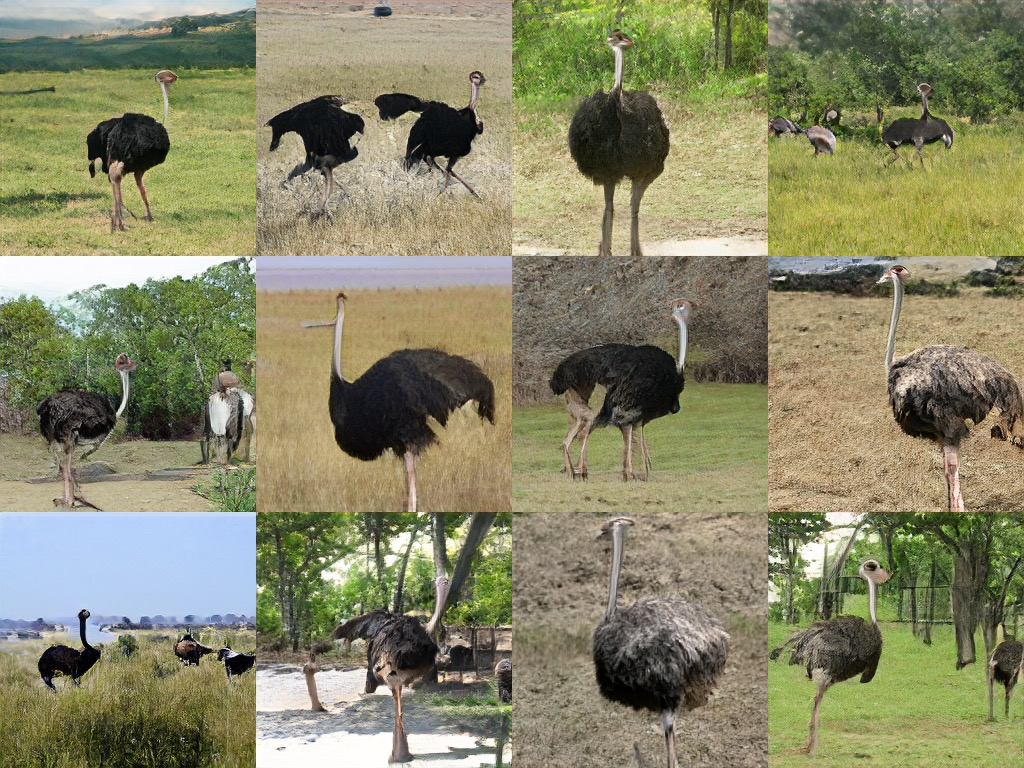
\includegraphics[ width=\tmpwidth]{figures/diversity/009_biggan_trun1.jpeg} & \hspace{-3mm}
    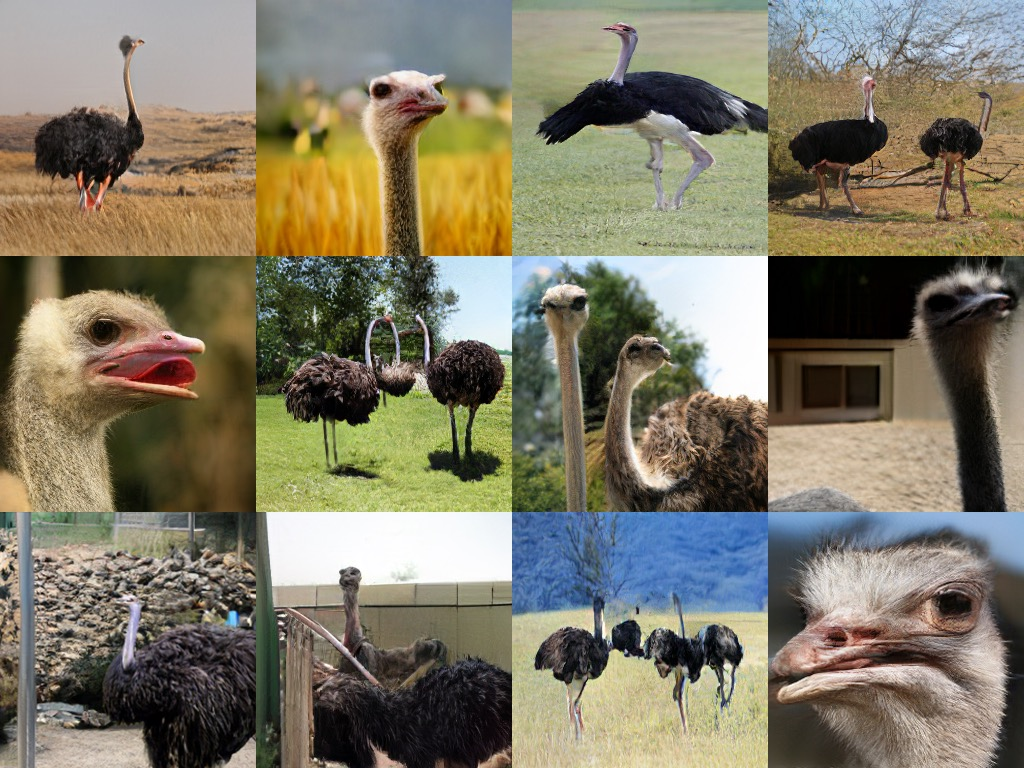
\includegraphics[ width=\tmpwidth]{figures/diversity/009_ours.jpeg} & \hspace{-3mm}
    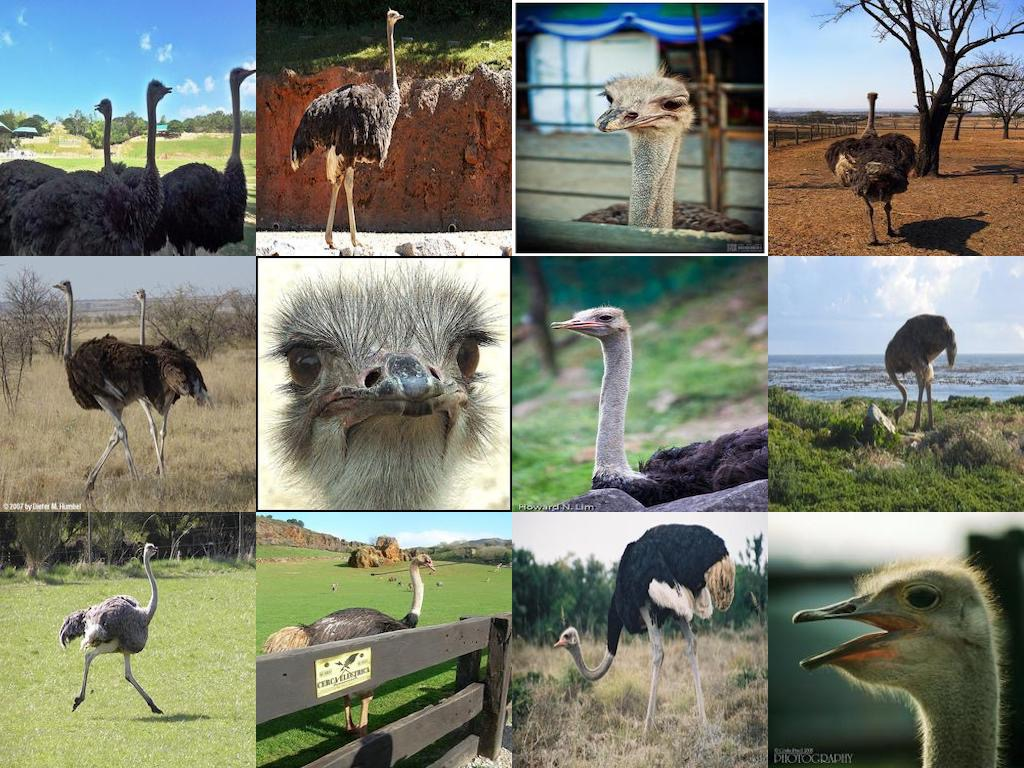
\includegraphics[ width=\tmpwidth]{figures/diversity/009_gt.jpeg} \\ 
    
    % \includegraphics[ width=\tmpwidth]{figures/diversity/130_biggan_trun1.jpeg} & \hspace{-3mm}
    % \includegraphics[ width=\tmpwidth]{figures/diversity/130_ours.jpeg} & \hspace{-3mm}
    % \includegraphics[ width=\tmpwidth]{figures/diversity/130_gt.jpeg} \\ 
 
    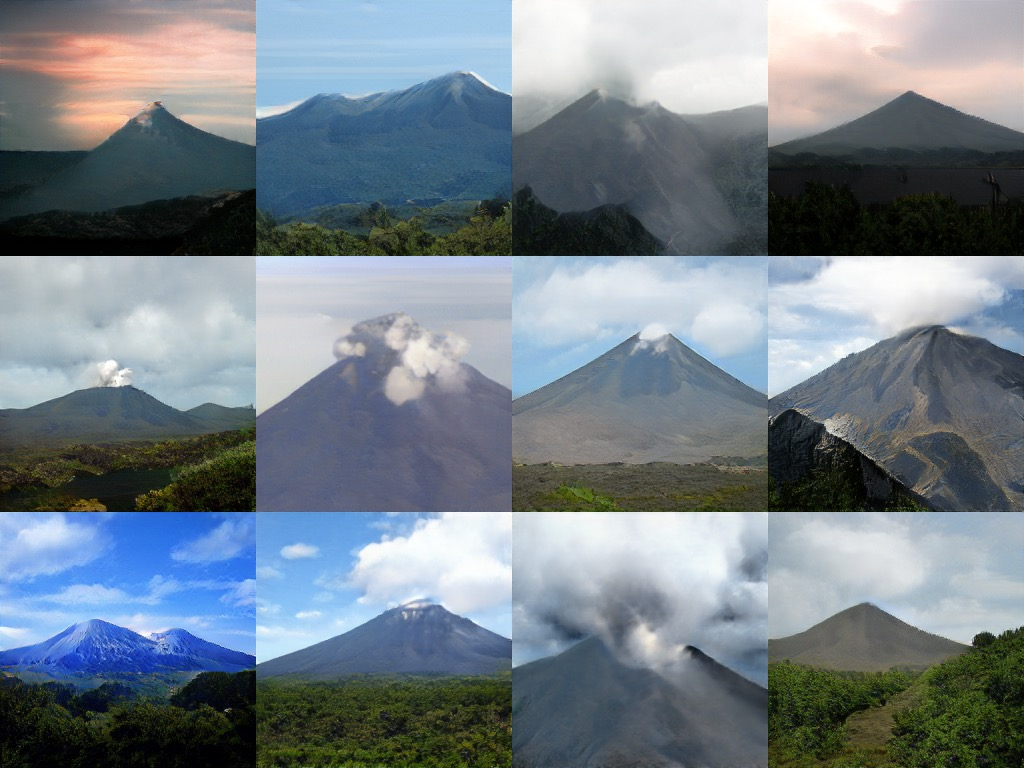
\includegraphics[ width=\tmpwidth]{figures/diversity/980_biggan_trun1.jpeg} & \hspace{-3mm}
    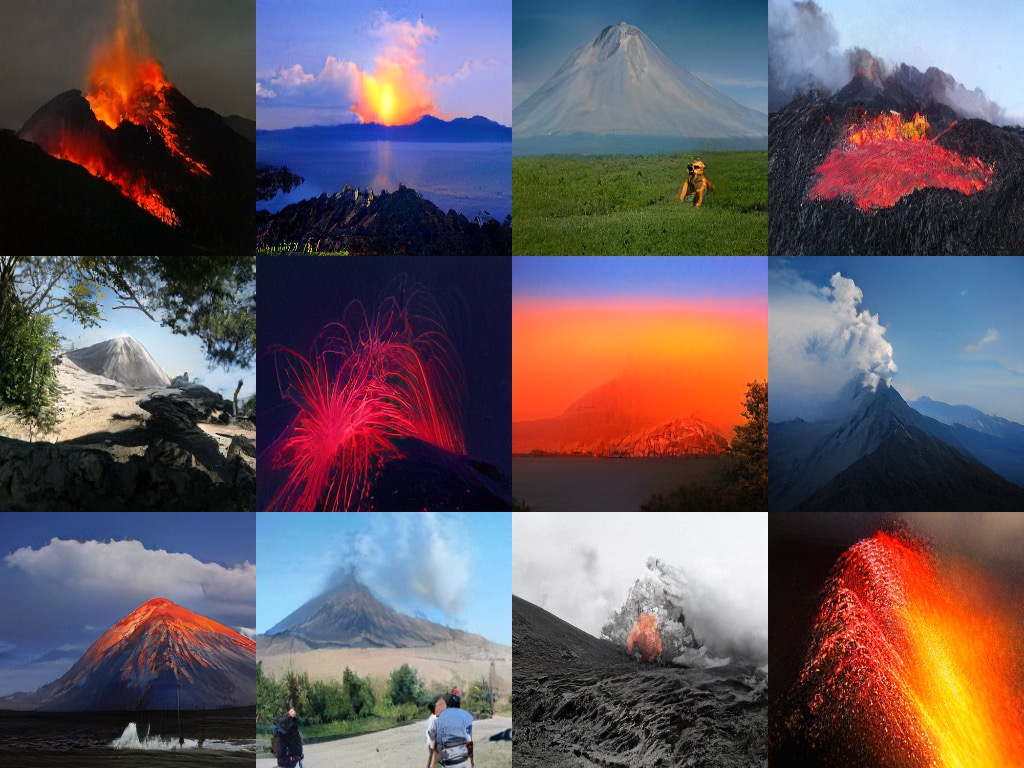
\includegraphics[ width=\tmpwidth]{figures/diversity/980_ours1.jpeg} & \hspace{-3mm}
    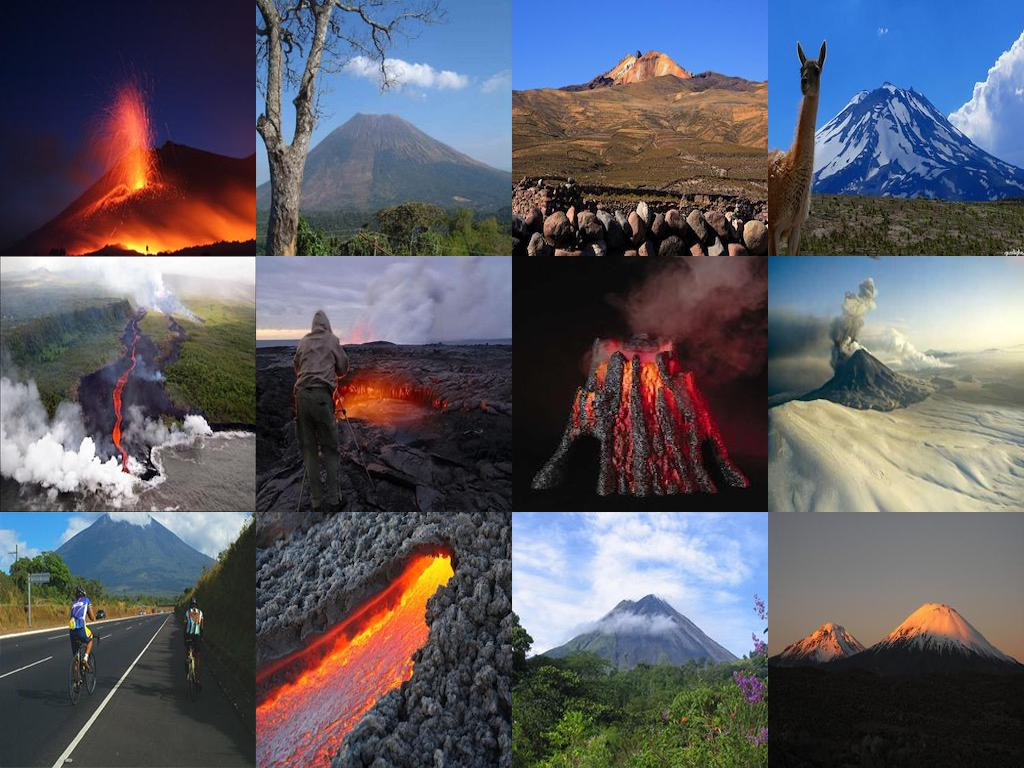
\includegraphics[ width=\tmpwidth]{figures/diversity/980_gt.jpeg} \\
    
    % \includegraphics[ width=\tmpwidth]{figures/diversity/145_biggan_trun1.jpeg} & \hspace{-3mm}
    % \includegraphics[ width=\tmpwidth]{figures/diversity/145_ours.jpeg} & \hspace{-3mm}
    % \includegraphics[ width=\tmpwidth]{figures/diversity/145_gt.jpeg} \\
    
    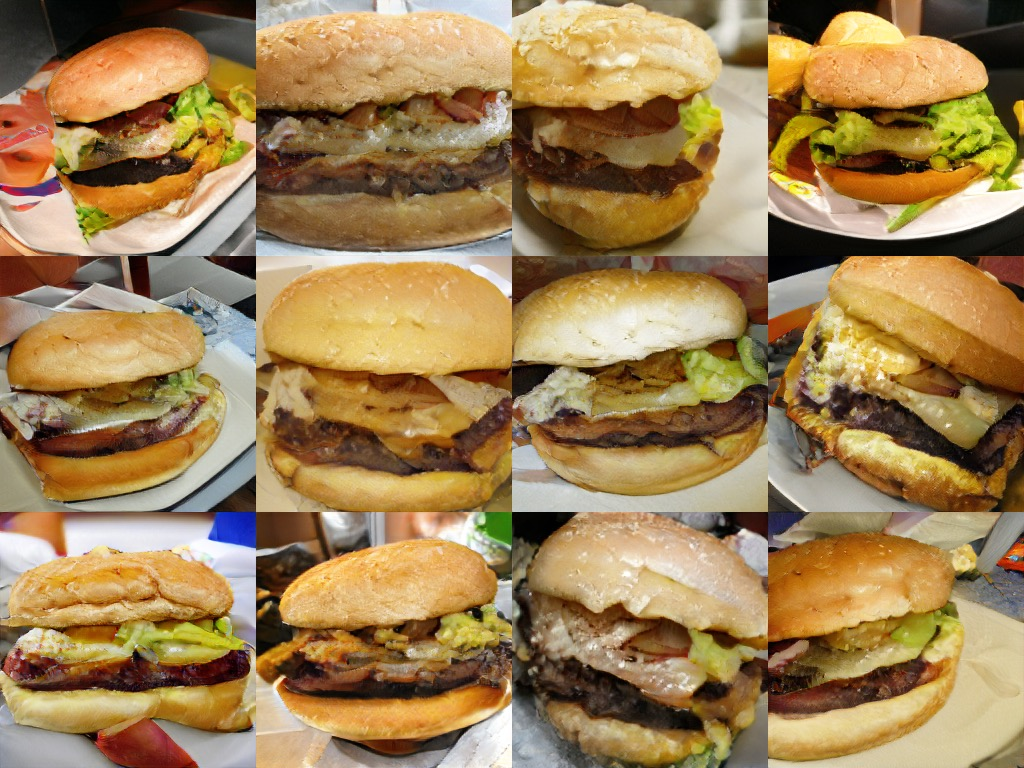
\includegraphics[ width=\tmpwidth]{figures/diversity/933_biggan_trun1.jpeg} & \hspace{-3mm}
    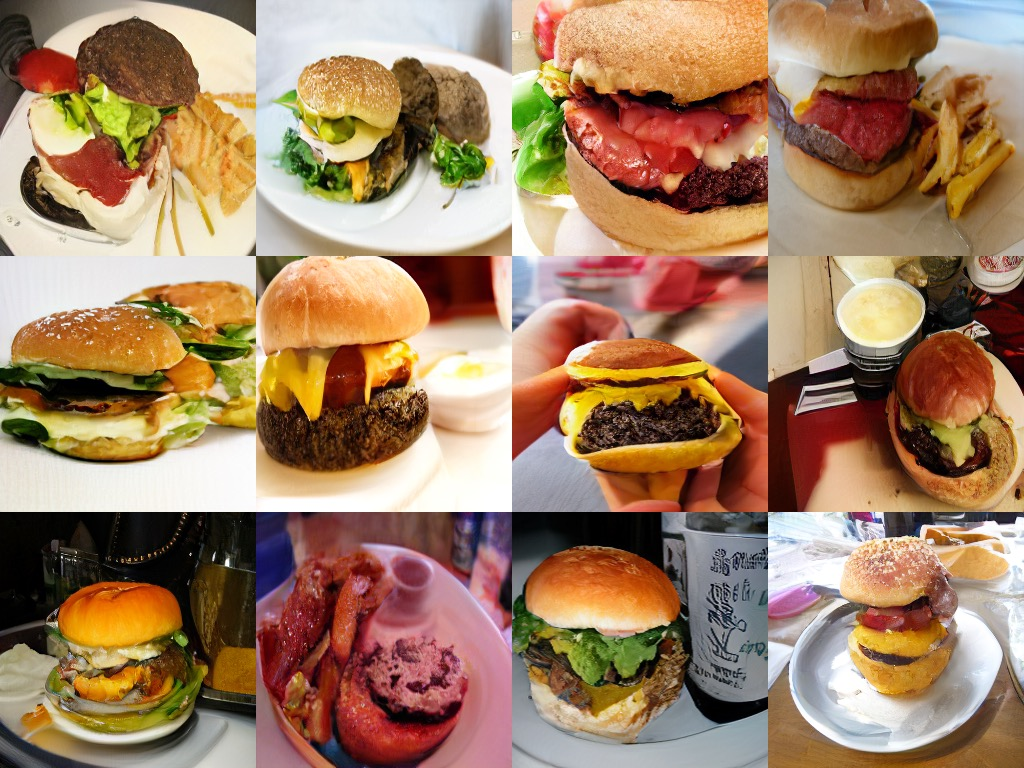
\includegraphics[ width=\tmpwidth]{figures/diversity/933_ours.jpeg} & \hspace{-3mm}
    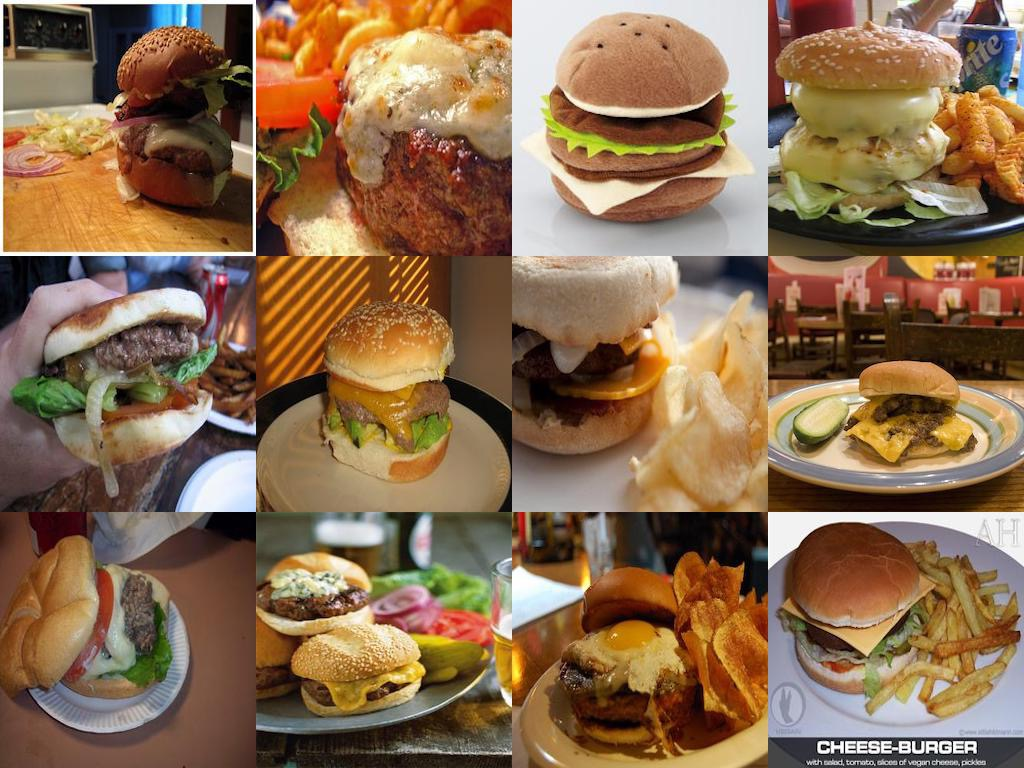
\includegraphics[ width=\tmpwidth]{figures/diversity/933_gt.jpeg} \\     

    % \includegraphics[ width=\tmpwidth]{figures/diversity/000_biggan_trun1.jpeg} & \hspace{-3mm}
    % \includegraphics[ width=\tmpwidth]{figures/diversity/000_ours1.jpeg} & \hspace{-3mm}
    % \includegraphics[ width=\tmpwidth]{figures/diversity/000_gt.jpeg} \\   
    
    BigGAN-deep (FID=$6.95$) & \model (FID=\bestfid) & Training Set \\
    \end{tabular}
    \vspace{-2mm}
    \caption{Sample Diversity Comparison between our proposed method \model and BigGAN-deep~\cite{biggan} on ImageNet 256$\times$256. 
    %BigGAN was sampled with $1.0$ truncation to yield the maximum diversity. In contrast to BigGAN's samples, our proposed method generate more diverse samples such as varied lighting, poses, scales and context, which are visually closer to the training set.
    The class ids of the samples from top to bottom  are {\footnotesize{ \texttt{009}}, \footnotesize{\texttt{980}} and \footnotesize{\texttt{993}}} respectively. Please refer to appendix for more comparisons.}
    \vspace{-6mm}
    \label{fig:diversity}
\end{figure*}